
\section{System}

In this section, we introduce the main components of the system. Our system is built with a pipeline architecture in mind giving it the advantage to run each section separately to allow stream processing without blocking the data flow of components (Figure~\ref{fig:system}). The three logical components include sections on \textit{Model} for entity resolution purposes, \textit{Wiki Citation} to annotate cite-worthy documents, \textit{Slot Filling} to generate the actual slot values.


To walk you through the steps we take, assume we only care about on single WP entity, the first step is to extract aliases of the entity. We use several approaches to get as many viable aliases as possible. Then we look into the stream of content that is being generated on the internet, apply two levels of filtering to finally end up with the documents are central to that entity. To extract the relevnat slot values we perform pattern matching in each sentence or coreferent sentence to see if we can find a match. As a match is found from the content of the sentence to the patterns that we have generated regarding slot name, the associated slot value is extracted as a final result.

%\ceg{Discuss current system first. If you want to keep the decisions points that led to the current architecture, make it a subsection.}

\begin{figure}
  \centering
%  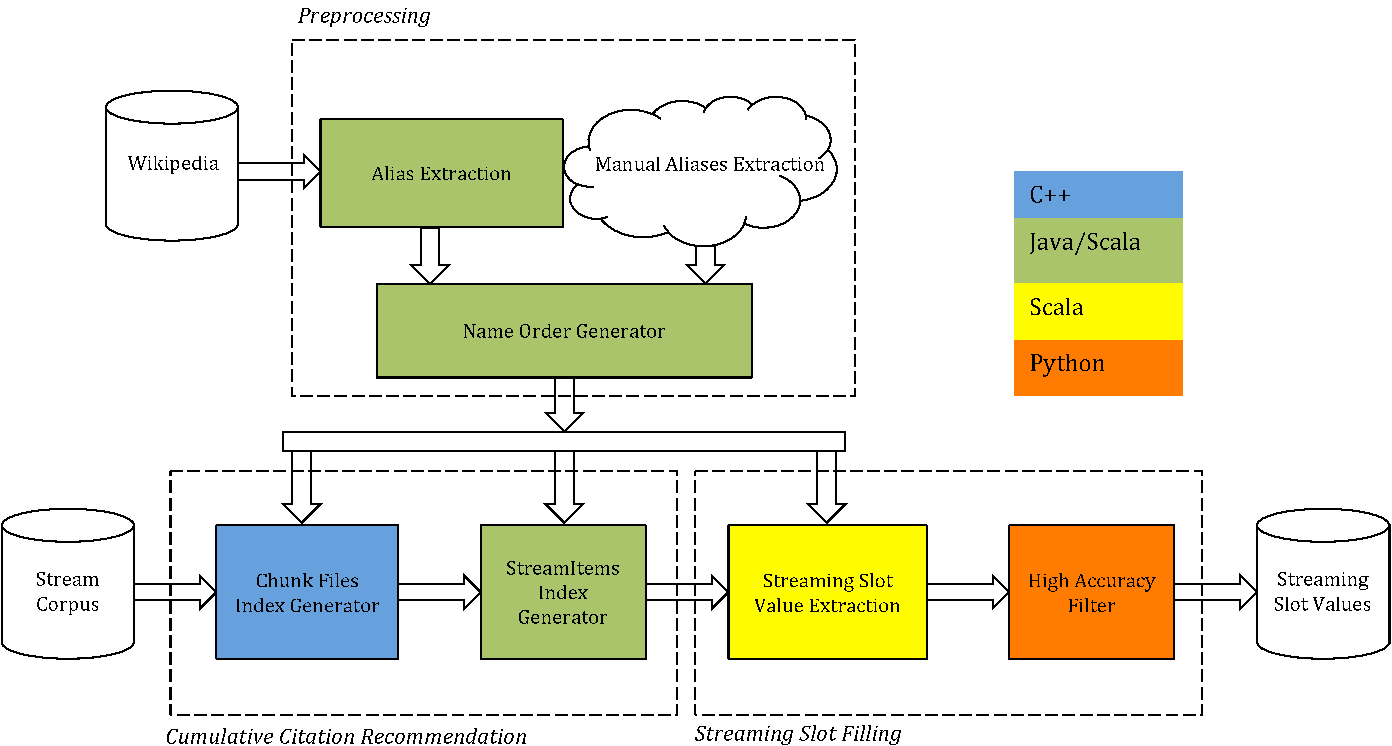
\includegraphics[width=6in]{./images/sdl-eps-converted-to.pdf}
  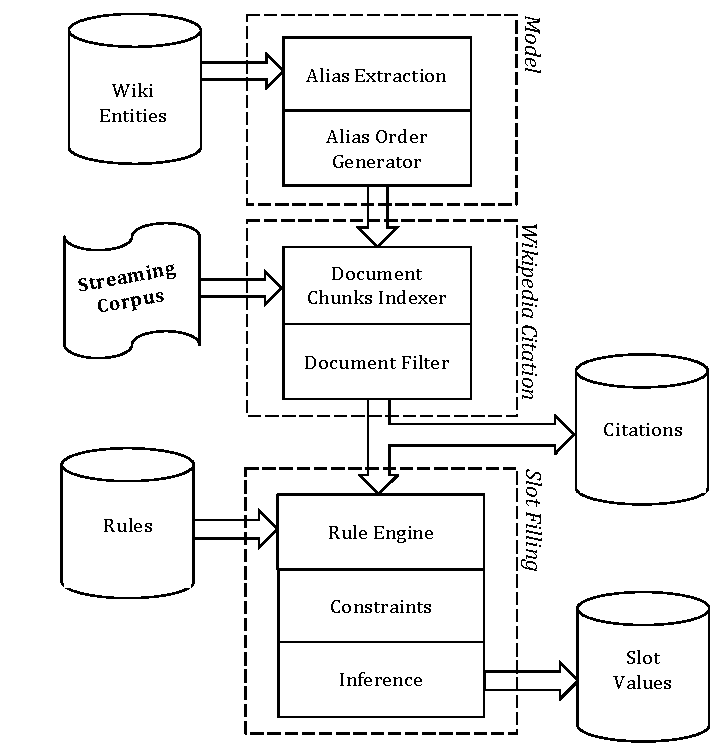
\includegraphics[width=3in]{./images/System_Diagram_with_model_Vertical-crop.pdf}
% http://convert.neevia.com/pdfconvert/
  \vspace*{-.1in} 
  \caption{System Architecture.
  Components are logical groups noted with dotted boxes.}
  \label{fig:system}
  \vspace*{-.2in}
\end{figure}



\subsection{Model}

We use Wikipedia API to get these aliases automatically. This is done by retrieving backlink references (redirects of a wiki entity), e.g. William Henry Gates is an alias for Bill Gates in WP as a backlink reference. Unfortunately this is not good enough and to enhance recall we need more aliases. To have better use of a wiki page we parse HTML DOM of the page, then use regular expressions to extract the bold phrases of the first paragraph as alias of the actual entity. Based on our observation this is a very accurate heuristic and provides us with lots of famous aliases of the entities. As an example of when this might not wirk, is that there might be occasions that some other topic is written in bold typesetting in the first paraph apart from the entity aliases itself but these are very rare.

Once aliases are available we pass them through rules of generating proper name orders which will produce various forms of writing a name. As a basic example Bill Gates can be written as Gates, Bill also. This will allow the system to capture various notation forms of aliases. We refer to this part as \textit{Alias Order Generator}.

\textit{Cumulative Citation Recommendation.}
The main goal of CCR is to have an aggregate list of documents that are worthy of being cited in a Wikipedia page. We perform exact string matching and treat all the documents that mention an entity equally likely to be citable. One of the reasons for this is that in former TREC KBA reports \cite{JFrank12} there were observations of how non-mentioning documents have a low chance of being citable in Wikipedia. So we take on that and ignore non-citing documents. 


% Note: Describe the algorithms of each phase
% Talk in abstract terms not implementation.
% Use formal representations (Math, SQL etc)


%\ceg{This section should be structured as follows:
%1: Introduce CCR (Motivation, Expectations)
%2: Our high level approach
%3: Discussion of our design (Like already discussed)
%}


\textit{Streaming Slot Filling.}
%\ceg{See the previous note.}
The purpose of SSF is to extract proper values for relations of interest, which can be found in Table~\ref{table:slotNameOntology}. This is called Stream Slot Filling because data is being generated as time goes
on and for each extraction we should only consider current or past data. In Figure~\ref{fig:system} we refer to this as \textit{Streaming Slot Value Extraction}. Stream slot filling is done by pattern matching documents with manually produced patterns for slots of interest. The way we do this is by observing a sentence that has a mention of the entity or one of its coreferences. An anchor word in the sentence related to the slot name is located and we match either left or right of the anchor word for potential slot values. 

\textit{Post Processing Algorithm.}
The SSF output of many extractions is noisy. The data contains duplicates and incorrect extractions. We can define rules to sanitize the output only using the information present in the SSF file. The file is processed in time order, in a tuple-at-a-time fashion to minimize the impact on accuracy. We define two classes of rules deduplication rules and inference rules. In our diagram we refer to this component as \textbf{High Accuracy Filter}.
